
% You may delete everything from \appendix up to \end{document} if you don't need it.
\appendix

\chapter{Appendix}

\section{Small vs Large Vocabulary}\label{app:small_vs_large_vocabulary}

\section{Chord Mapping}\label{app:chord_mapping}

Chords in Harte notation were mapped to the vocabulary with $C=170$ by first converting them to a tuple of integers using the Harte library. These integers represent pitch classes and are in the range 0 to 11 inclusive. They are transposed such that 0 is the root pitch. These pitch classes were then matched to the pitch classes of a quality in the vocabulary, similar to the work by \citet{StructuredTraining}. However, for some chords, this was not sufficient. For example, a \texttt{C:maj6(9)} chord would not fit perfectly with any of these templates due to the added 9th. Therefore, the chord was also passed through Music21's~\citep{music21} chord quality function which matches chords such as the one above to major. This function would not work alone as its list of qualities is not as rich as the one defined above. If the chord was still not matched, it was mapped to \texttt{X}. This additional step is not done by \citet{StructuredTraining} but gives more meaningful labels to roughly one third of the chords previously mapped to \texttt{X}.

\section{CRNN with CR2}\label{app:crnn_with_cr2}

\begin{table}[H]
    \centering
    \begin{tabular}{lccccccc}
        \toprule
        cr2 & acc & root & third & seventh & mirex & acc\textsubscript{class} & median\textsubscript{class} \\  
        \midrule
        on & 59.7 & \textbf{78.9} & \textbf{75.6} & 61.9 & \textbf{80.5} & 18.4 & 0.4 \\
        off & \textbf{60.2} & 78.4 & 75.3 & \textbf{62.5} & 79.5 & \textbf{19.4} & \textbf{1.1} \\
        \bottomrule
    \end{tabular}
    \caption{\emph{CRNN} with and without the added `CR2' decoder. Performance is very similar between the two. It could be argued that te model with CR2 on is better, but for simplicity, I proceed with the model without CR2. One could also argue that the effect of CR2 is similar to simply adding more layers to the GRU already present in \emph{CRNN}.}
\end{table}

\section{A Long Run with SGD}\label{app:long_sgd}
\begin{figure}[H]
    \centering
    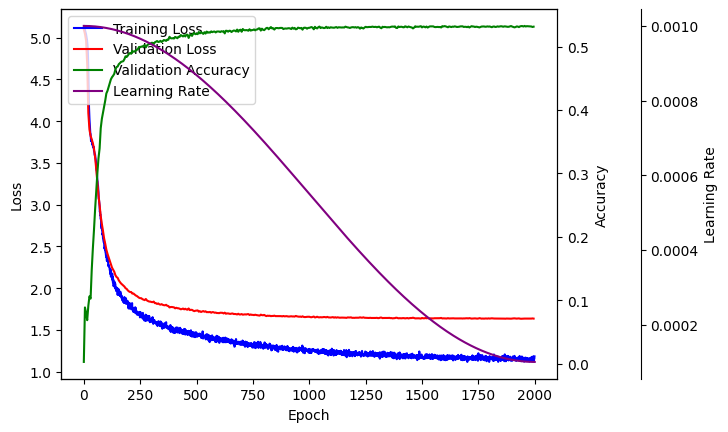
\includegraphics[width=1.0\textwidth]{figures/long_sgd_training_plot.png}
    \caption{Training graphs for \emph{CRNN} trained with SGD, momentum 0.9, a learning rate of $0.001$ and the \texttt{cosine} scheduling for 2000 epochs. Convergence is reached but performance does not exceed that which is achieved by Adam over 150 epochs. Furthermore, there is signifcant computational cost associated with running for 2000 epochs. I proceed with Adam for the remainder of experiments. }\label{fig:long_sgd}
\end{figure}


\section{Random Hyperparameter Search Sets}\label{app:random_hyperparameter_search_sets}

$\texttt{hidden\_size}\in\{32,33,\ldots,512\}$, $\texttt{num\_layers}\in\{1,2,3\}$, $\texttt{segment\_length}\in\{5,6,\ldots,45\}$, $\texttt{kernel\_size}\in\{5,6,\ldots,15\}$, $\texttt{cnn\_layers}\in\{1,2,\ldots,5\}$ and $\texttt{cnn\_channels}\in\{1,2,\ldots,5\}$

% \section{CNN Hyperparameter Search}\label{app:cnn_hparams}

% \begin{table}[H]
%     \centering
%     \begin{tabular}{@{}cccccccccc@{}}
%         \toprule
%         $k$ & $l$ & $c$ & acc & root & third & seventh & mirex & acc\textsubscript{class} & median\textsubscript{class} \\  
%         \midrule
%         5 & 1 & 1 & 54.5 & 74.4 & 69.0 & 56.6 & 73.5 & 16.0 & 2.3 \\
%         5 & 3 & 5 & 57.0 & 76.9 & 72.5 & 59.2 & 77.6 & 18.9 & 3.0 \\
%         9 & 5 & 10 & \textbf{57.8} & \textbf{78.1} & \textbf{74.0} & \textbf{60.0} & \textbf{77.8} & \textbf{19.2} & \textbf{3.2} \\
%         \bottomrule
%     \end{tabular}
%     \caption{CNN hyperparameter search results. The best performing result for each metric is highlighted in \textbf{bold}. Performance increases with depth of the model. However, the performance increase is not significant between the two best performing models. Deeper CNNs were also trained, but were results did not improve and were too computationally intensive to run repeatedly.}
% \end{table}

\section{Confusion Matrix of CRNN over Roots}\label{app:cm_roots}

\begin{figure}[H]
    \centering
    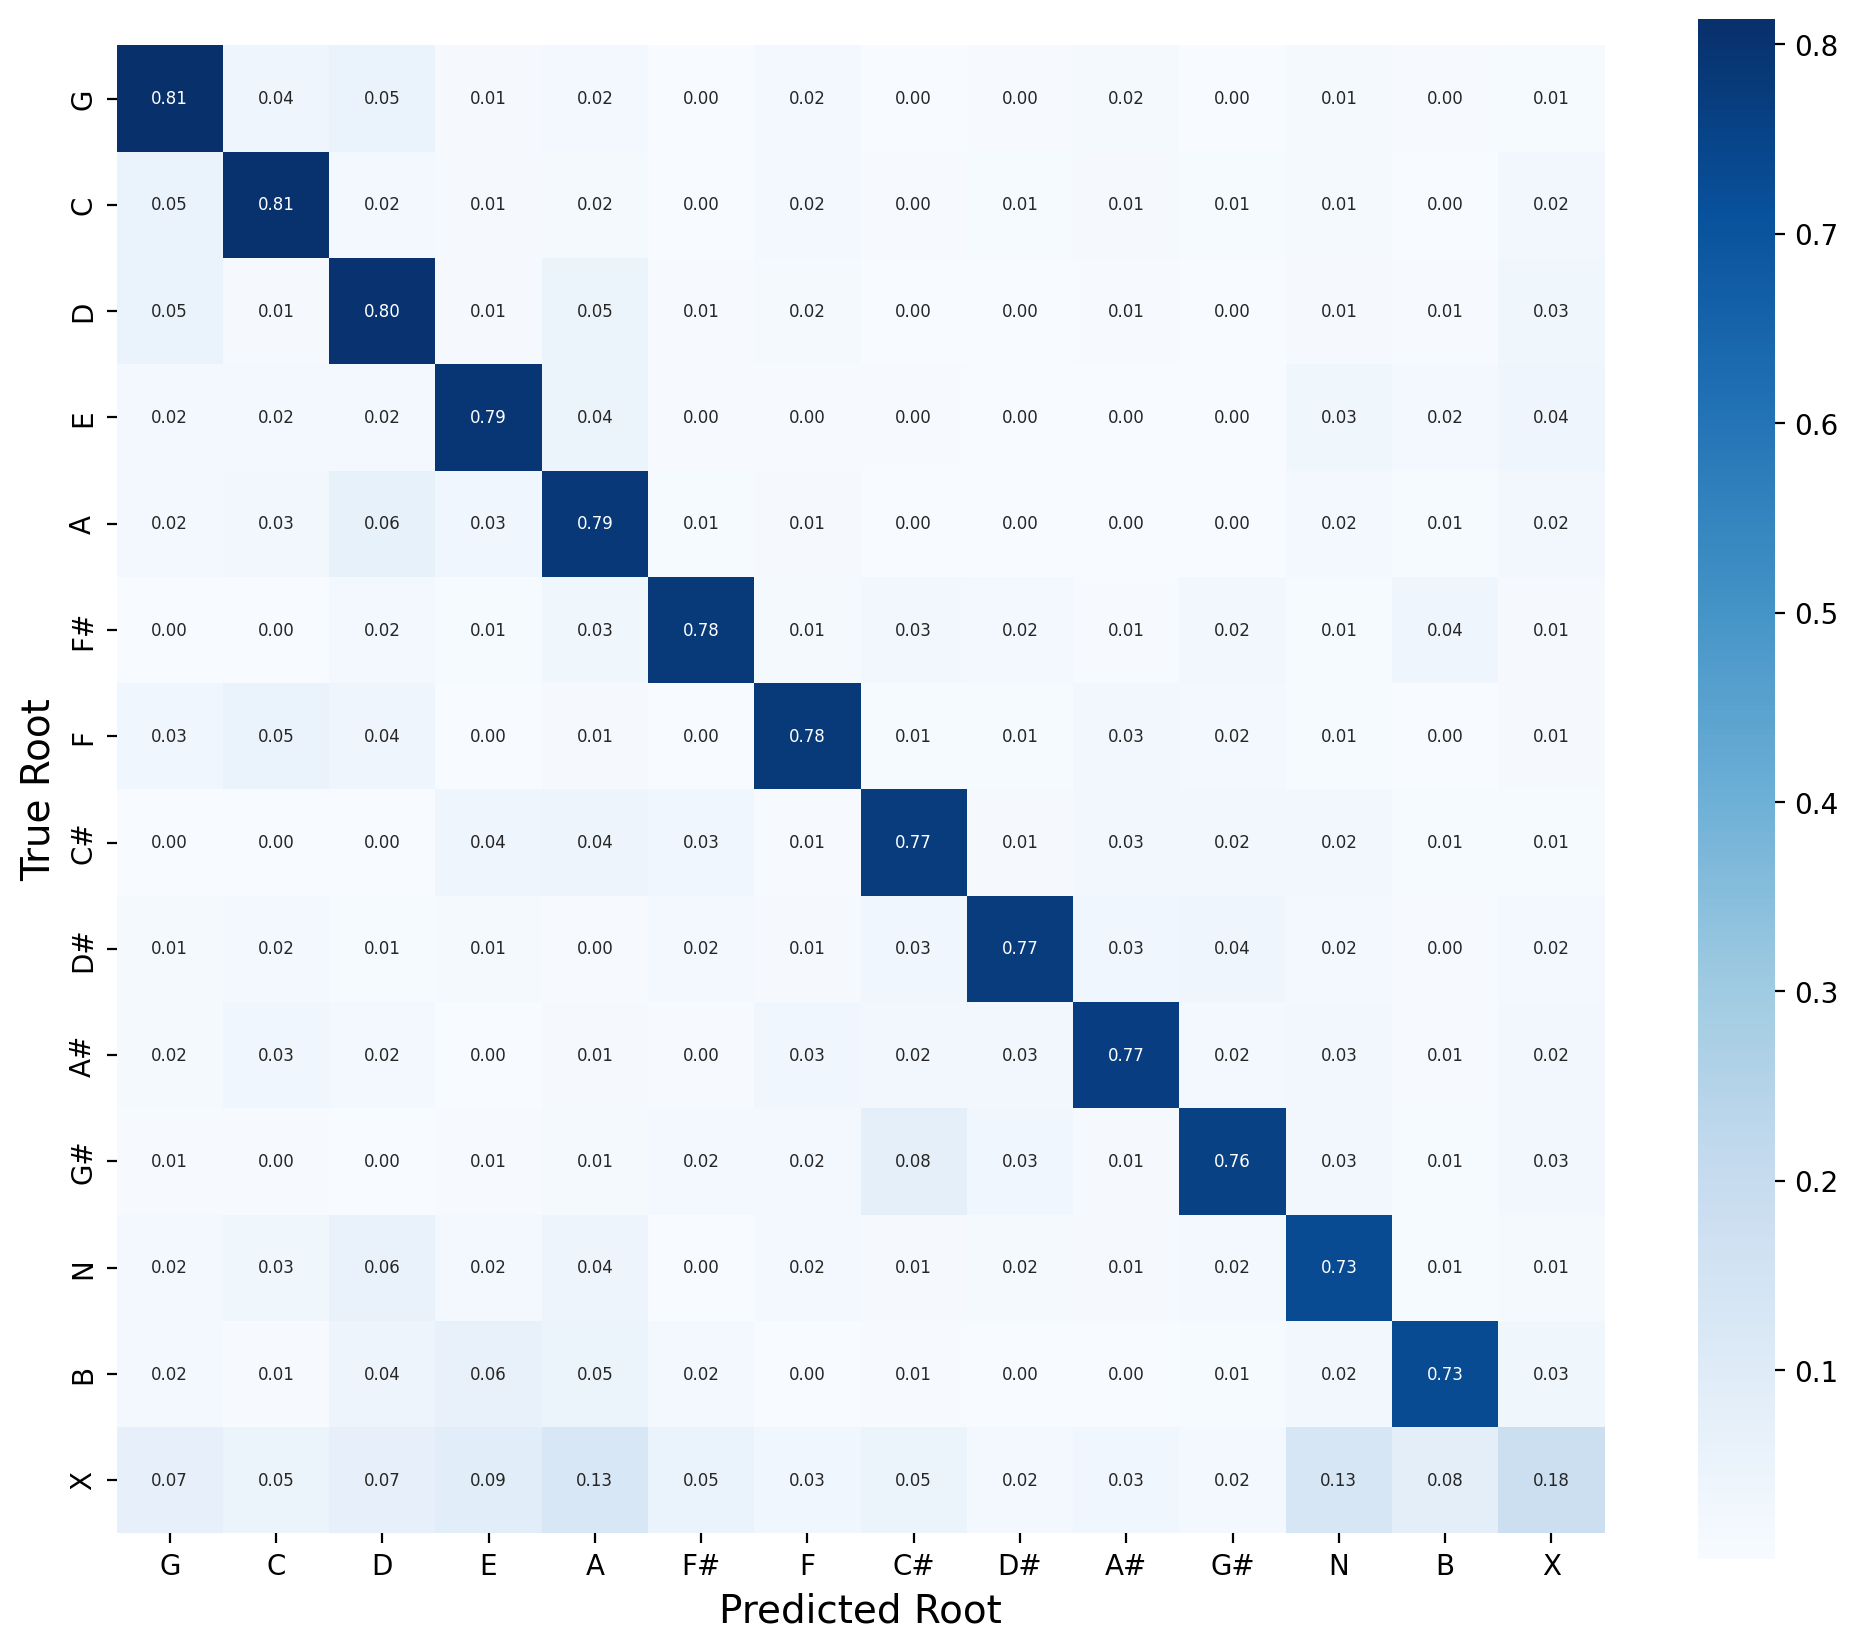
\includegraphics[width=1.0\textwidth]{figures/confusion_matrix_roots.png}
    \caption{Performance is relatively stable across roots. The only outlier is the unknown chord symbol \texttt{X}. This is to bexpected given the ambiguous nature of the chord. }
    \label{fig:cm_roots}
\end{figure}

% \section{Accuracy vs Hop Length}\label{app:accuracy_vs_hop_length}

% \begin{figure}[H]
%     \centering
%     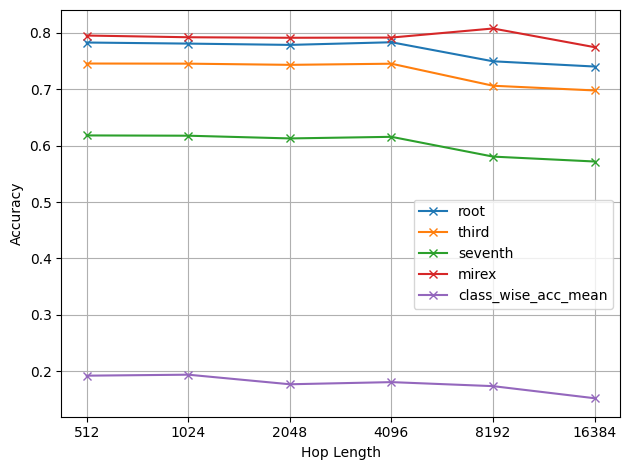
\includegraphics[width=0.5\textwidth]{figures/hop_length_vs_accuracy.png}
%     \caption{Accuracy vs hop length. Metrics are not directly comparable over hop lengths due to different likelihoods. However, the metrics are fairly consistent over different hop lengths, certainly over the region explored by the literature $[512,2048,4096]$. Every hop length tested is short enough to be more granular than chords, but not so short that the computed CQT is too noisy. We continue with the default hop length of $4096$, to be consistent with some of the literature while keeping computational cost low.}
%     \label{fig:accuracy_vs_hop_length}
% \end{figure}

\section{Incorrect Region Lengths With/Without Smoothing}\label{app:histogram_over_region_lengths}

\begin{figure}[H]
    \centering
    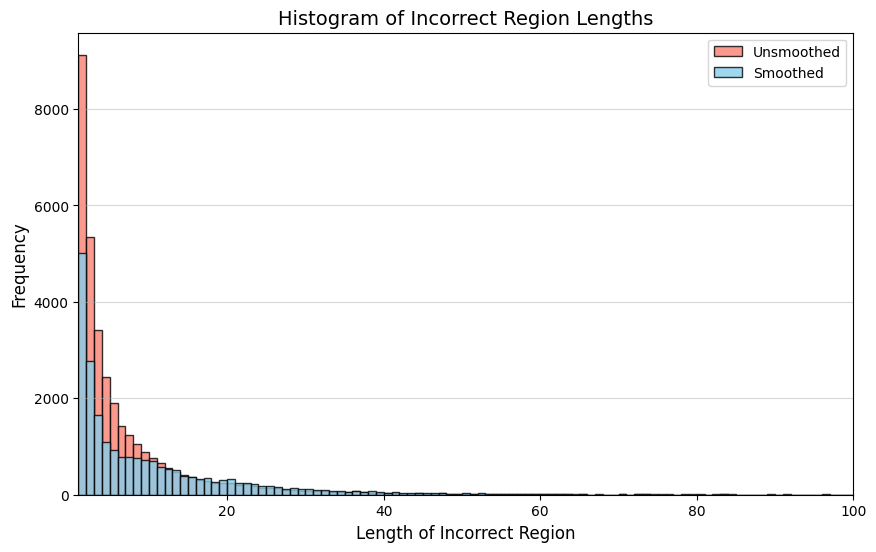
\includegraphics[width=0.6\textwidth]{figures/incorrect_region_smoothing_histogram.png}
    \caption{Histogram over incorrect region lengths for a \emph{CRNN} with and without smoothing. An incorrect region is defined as a sequence if incorrect frames with correct adjacent of either end. Both distributions have a long-tail, with $26.7\%$ regions being of length 1 without smoothing. This raises concerns over the smoothness of outputs and requires some form of post-processing explored in Section~\ref{sec:decoding}. The distribution is more uniform with smoothing, with approximately half the very short incorrect regions.}
    \label{fig:histogram_over_region_lengths}
\end{figure}

\section{Accuracy over the Context}\label{app:accuracy_over_context}
\begin{figure}[H]
    \centering
    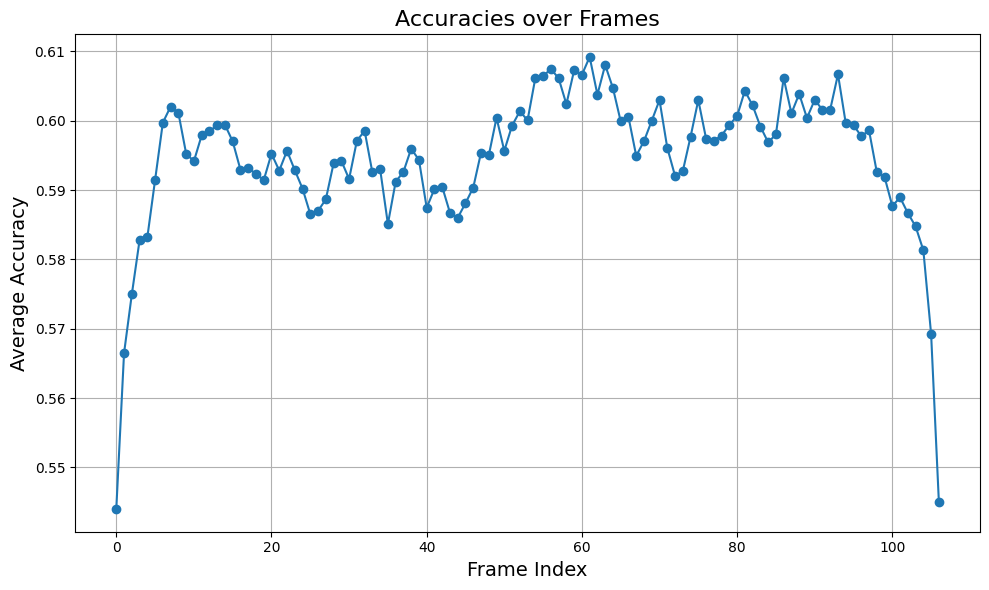
\includegraphics[width=0.8\textwidth]{figures/accuracy_over_frames.png}
    \caption{Average frame-wise accuracy of the \emph{CRNN} model over the patch of audio. The model performs worse at the beginning and end of the patch of audio, as expected. However, the differences are only $~0.05$. We propose that the context on one side is enough for the model to attain the vast majority of the performance attained with bi-directional context. This plot supports our procedure of evaluating over the entire song at once. }\label{fig:crnn_context}
\end{figure}

\section{Accuracy vs Context Length of Evaluation}\label{app:accuracy_vs_context_length}

\begin{figure}[H]
    \centering
    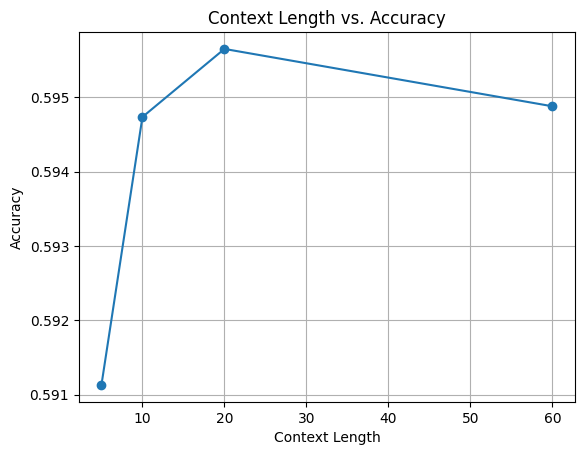
\includegraphics[width=0.5\textwidth]{figures/context_length_vs_accuracy.png}
    \caption{Accuracy with increasing segment length of validation set. The accuracy increases very slightly. I choose to continue evaluating over the entire song at once.}
    \label{fig:accuracy_vs_context_length}
\end{figure}